\section{Working in Kubernetes}

\subsection{Objectives}
	\begin{frame}
		\frametitle{Objective}
		Now that we have a worker, we want to run it in a kubernetes cluster.
		
		\bigskip
		The first step will be to run a container into kubernetes to make sure that we can do it.
		
		Then, we will run our worker in kubernetes.	
	\end{frame}
	
\subsection{Configure our environment}
	
	\begin{frame}
		\frametitle{How to access to a Kubernetes cluster}
		
		The kubectl client used to access a kubernetes cluster used the configuration file \$home/.kube/config
		
		More informations \href{https://kubernetes.io/docs/tasks/access-application-cluster/configure-access-multiple-clusters/}{here}.
		
		\bigskip
		
		If we are using Minikube, starting it already configure kubectl.
		
		\bigskip
		
		As indicated in \href{https://kubernetes.io/docs/tasks/tools/install-kubectl/\#enabling-shell-autocompletion}{this documentation}, you can activated the completion for kubectl.
		
	\end{frame}
	
	\begin{frame}[fragile]
		\frametitle{Working in a dedicated namespace}
		
		To avoid impacting other components, we are going to isolate ourselves in a namespace:
		\begin{block}{Command line}
			\begin{verbatim}
				kubectl get namespaces
				kubectl create namespace my-namespace
				kubectl get ns
			\end{verbatim}
		\end{block}
	\end{frame}
		
	\begin{frame}[fragile]
		\frametitle{Working in a dedicated namespace}
	
		Then we configure kubectl to use his context:
		\begin{block}{Command line}
			\begin{small}
			\begin{verbatim}
					kubectl config get-context
				
					kubectl config set-context training        \
					                   --cluster=kubernetes    \
					                   --user=kubernetes-admin \
					                   --namespace=my-namespace
							
					kubectl config use-context training
					kubectl config get-context
				\end{verbatim}
			\end{small}
		\end{block}
		In \textbf{minikube}, replace \textit{kubernetes} cluster and \textit{kubernetes-admin} user by \textit{minikube}.
	\end{frame}
	
\subsection{Run a container in kubernetes}	
		
	\begin{frame}[fragile]
		\frametitle{Running our first container in the cluster}
	
		To begin, we are just going to deploy a container sending a ping:
		\begin{block}{Command line}
			\begin{verbatim}
				kubectl run pingpong --image=alpine ping 1.1.1.1
				
				kubectl get pods
				kubectl get deployments -o wide
				kubectl get replicaset -o wide
			\end{verbatim}
		\end{block}
	\end{frame}
	
	\begin{frame}
		\frametitle{Kubernetes application architecture}
		
		\begin{center}
		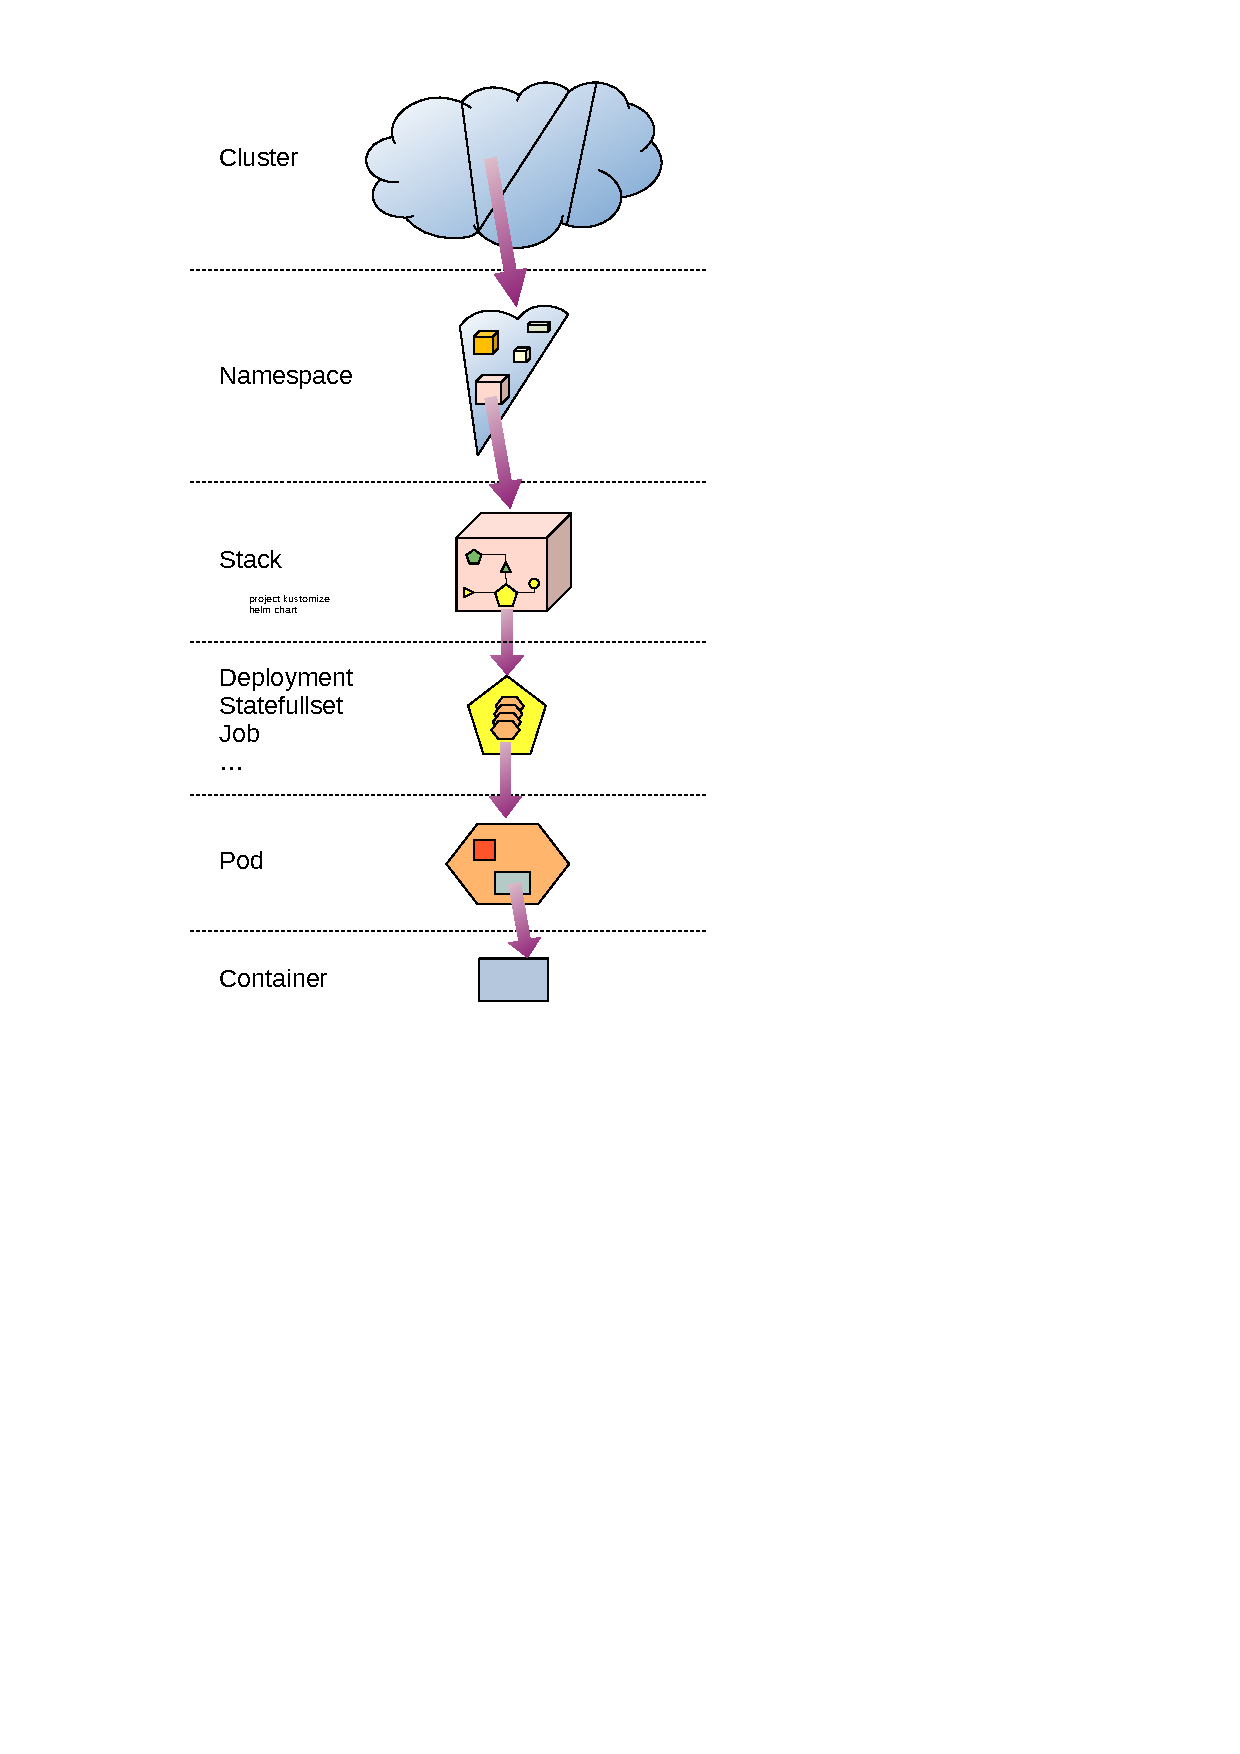
\includegraphics[height=11.5cm]{../../../resources/color/fromCluster2container.pdf}
		\end{center}
		
	\end{frame}		

	\begin{frame}
		\frametitle{Prepare the environment}
		
		Starting from now, we are going to use 3 shell in 3 differents windows/panes.
		
	\end{frame}		

	\begin{frame}[fragile]
		\frametitle{Looking at logs in a kubernetes cluster}
	
		We want to display the logs of this container:
		\begin{block}{Command line in window 1}
			\begin{verbatim}
				kubectl logs -f pingpong-XXXX-XXXX
			\end{verbatim}
		\end{block}
		
		Something happens and we need to recreate the pod:
		\begin{block}{Command line in window 2}
			\begin{verbatim}
				kubectl get pods -w
			\end{verbatim}
		\end{block}
		\begin{block}{Command line in window 3}
			\begin{verbatim}
				kubectl delete pod pingpong-XXXX-XXXX
			\end{verbatim}
		\end{block}
	\end{frame}
	
	\begin{frame}[fragile]
		\frametitle{Looking at logs in a kubernetes cluster}
	
		There are several problems:
		\begin{itemize}
			\item[$\bullet$] we do not see which logs comes from which pod
			\item[$\bullet$] in fact we do not see the new containers logs
			\item[$\bullet$] the follow is broken by the operation
		\end{itemize}
		
		How to solve this and be able to follow logs even if pods are moving?
	\end{frame}

	\begin{frame}[fragile]
		\frametitle{Using stern to look at logs}

		So, we are going to redo the operation but this time using stern:
		\begin{block}{Command line in window 1}
			\begin{verbatim}
				stern pingpong
			\end{verbatim}
		\end{block}
				\begin{block}{Command line in window 2}
			\begin{verbatim}
				watch kubectl get all
			\end{verbatim}
		\end{block}
		\begin{block}{Command line in window 3}
			\begin{verbatim}
				kubectl delete pod pingpong-XXXX-XXXX
			\end{verbatim}
		\end{block}
	\end{frame}
	
	\begin{frame}[fragile]
		\frametitle{Clean the namespace}
		
		Before returning to our worker, a little cleaning can be wise:
		\begin{block}{Command line in window 1}
			\begin{verbatim}
				kubectl delete deployment pinpong
				kubectl get all
			\end{verbatim}
		\end{block}
		
		\medskip
		
		And stop the commands in the other windows.
	\end{frame}
	
\subsection{Run our worker in kubernetes}

	\begin{frame}[fragile]
		\frametitle{Running our worker in kubernetes}
		
		Now that we know how to run something in kubernetes, we are going to do it with our worker:
		\begin{block}{Command line in window 2}
			\begin{verbatim}
				stern worker
			\end{verbatim}
		\end{block}		
		\begin{block}{Command line in window 3}
			\begin{verbatim}
				kubectl get pods -w
			\end{verbatim}
		\end{block}
		\begin{block}{Command line in window 1}
			\begin{verbatim}
				docker images
				docker build -t tinkou/worker:v1 .
				kubectl run worker --image=tinkou/worker:v1
			\end{verbatim}
		\end{block}
	\end{frame}
	
	\begin{frame}[fragile]
		\frametitle{Troubleshooting}
		
		Kubectl get pods indicate that something went wrong.
		
		Check kubernetes object to find the problem root cause:
		\begin{block}{Command line in window 1}
			\begin{verbatim}
				kubectl	describe deployment worker
				kubectl describe replicaset worker-XXXX
				kubectl describe pod worker-XXXX-XXXX
			\end{verbatim}
		\end{block}
		
	\end{frame}
	
	\begin{frame}[fragile]
		\frametitle{Using a registry}
		
		As our cluster can't access our local image, let's push it in a repository instead:
		\begin{block}{Command line 1}
			\begin{verbatim}
				docker tag tinkou/worker:v1 \
				           <registry>/training/worker-<id>:v1
				docker login <registry>
				docker push <registry>/training/worker-<id>:v1
			\end{verbatim}
		\end{block}
		\verb|<registry>| is the registry given by your sysadmin.
		
		\verb|<id>| is used to differenciate the images between the different trainees.

	\end{frame}
	
	\begin{frame}[fragile]
		\frametitle{Using a registry}
	
		And we try again by forcing a pod reconstruction::
		\begin{block}{Command line 1}
			\begin{verbatim}
				kubectl edit deployment worker
			\end{verbatim}
			\medskip
			And change the image field value.
		\end{block}
	
	\end{frame}

	\begin{frame}[fragile]
		\frametitle{Adding docker registry credentials}
		
		The logs on the pod indicate that docker registry credentials aren't valid.
		
		We need to store in a kubernetes secret our registry credentials:
		\begin{block}{Command line 1}
			\begin{verbatim}
				kubectl create secret docker-registry regcred \
				        --docker-server=<registry>            \
				        --docker-username=<user>              \
				        --docker-password=<password>          \
				        --docker-email=<yourEmail>
			\end{verbatim}
		\end{block}
	\end{frame}
	
	\begin{frame}[fragile]
		\frametitle{Adding docker registry credentials}
		
		Get our worker deployment yaml and add to it these credentials:
		\begin{block}{Command line 1}
			\begin{verbatim}
				kubectl get deployment worker -o yaml >deployment.yaml
			\end{verbatim}
		\end{block}
		\begin{block}{deployment.yaml}
			\begin{verbatim}
				spec:
				  template:
				    spec:
				      imagePullSecrets:
				      - name: regcred
			\end{verbatim}
		\end{block}
	\end{frame}
	
	\begin{frame}[fragile]
		\frametitle{Adding docker registry credentials}
		And apply it to update the configuration:
		\begin{block}{Command line 1}
			\begin{verbatim}
				kubectl apply -f deployment.yaml
			\end{verbatim}
		\end{block}
	\end{frame}
